\documentclass[11 pt]{article}


% More symbols
%\usepackage{amsmath}
%\usepackage{amssymb}
%\usepackage{latexsym}

% Surround parts of graphics with box
\usepackage{boxedminipage}

% Package for including code in the document
\usepackage{listings}

% If you want to generate a toc for each chapter (use with book)
\usepackage{minitoc}

% This is now the recommended way for checking for PDFLaTeX:
\usepackage{ifpdf}

%% \newif\ifpdf
%% \ifx\pdfoutput\undefined
%% \pdffalse % we are not running PDFLaTeX
%% \else
%% \pdfoutput=1 % we are running PDFLaTeX
%% \pdftrue
%% \fi

\ifpdf
\usepackage[pdftex]{hyperref}
\fi

\ifpdf
\usepackage[pdftex]{graphicx}
\else
\usepackage{graphicx}
\fi


\setlength{\oddsidemargin}{-.45in}
\setlength{\evensidemargin}{-.5in} \setlength{\textwidth}{7.1in}
\setlength{\topmargin}{-.5in} \setlength{\textheight}{9.5in}

\usepackage{amssymb}
\usepackage[pdftex]{graphicx}
\usepackage{latexsym}
\usepackage{amsfonts}
\usepackage{amsmath}
\usepackage{amsthm}
\usepackage{multicol}

\pagestyle{empty}

\newtheorem{theorem}{Theorem}[section]
\newtheorem{algorithm}[theorem]{Algorithm}
\newtheorem{axiom}[theorem]{Axiom}
\newtheorem{case}[theorem]{Case}
\newtheorem{claim}[theorem]{Claim}
\newtheorem{conclusion}[theorem]{Conclusion}
\newtheorem{condition}[theorem]{Condition}
\newtheorem{conjecture}[theorem]{Conjecture}
\newtheorem{corollary}[theorem]{Corollary}
\newtheorem{criterion}[theorem]{Criterion}
\newtheorem{definition}[theorem]{Definition}
\newtheorem{example}[theorem]{Example}
\newtheorem{exercise}[theorem]{Exercise}
\newtheorem{lemma}[theorem]{Lemma}
\newtheorem{notation}[theorem]{Notation}
\newtheorem{problem}[theorem]{Problem}
\newtheorem{proposition}[theorem]{Proposition}
\newtheorem{solution}[theorem]{Solution}
\newtheorem{summary}[theorem]{Summary}
\newtheorem{mapping}[theorem]{Mapping}
\newtheorem{at}{Theorem}



\linespread{1.25}
%%\linespread{2.0}
\renewcommand{\Im}{\text{Im}}
\renewcommand{\Re}{\text{Re}}
\newcommand{\R}{\mathbb R} %%real numbers
\newcommand{\Q}{\mathbb Q} %%rational numbers
\newcommand{\Z}{\mathbb Z} %%integers
\newcommand{\E}{\mathcal E}
\newcommand{\M}{\mathcal M} %%measurable sets
\newcommand{\N}{\mathbb N}  %%natural numbers
\renewcommand{\L}{\mathcal L}
\renewcommand{\P}{\mathcal P}  %%power set
\renewcommand{\O}{\mathcal O}
\newcommand{\C}{\mathbb C}
\newcommand{\J}{\mathbb J}
\renewcommand{\S}{\Sigma}
\newcommand{\B}{\mathcal B}
\newcommand{\T}{\mathcal T}  %%topology
\newcommand{\A}{\mathcal A}
\newcommand{\nullset}{\varnothing}
\newcommand{\sub}{\subseteq}
\newcommand{\U}{\mathcal U}
\renewcommand{\o}{\overline}



%%vectors in R^n
\renewcommand{\a}{\alpha}
\renewcommand{\b}{\mathbf b}
\newcommand{\x}{\mathbf x}
\newcommand{\y}{\mathbf y}
\newcommand{\z}{\mathbf z}
\newcommand{\D}{\mathcal D}

\renewcommand{\bf}{\textbf}
\newcommand{\mbf}{\mathbf}
\newcommand{\bmat}{\begin{bmatrix}}
\newcommand{\emat}{\end{bmatrix}}

\newcommand{\e}{\varepsilon} %% epsilon
\renewcommand{\d}{\delta}  % delta
\renewcommand{\r}{\rho}
\newcommand{\s}{\sigma}
\renewcommand{\t}{\theta}
\newcommand{\p}{\phi}
\newcommand{\ds}{\displaystyle}
\renewcommand{\mod}{\text{mod }} %% modulo
\newcommand{\dist}{\text{dist}}
\newcommand{\Ran}{\text{Ran }}
\newcommand{\Res}{\text{Res}}

\newcommand{\response}{\vspace{.2in}}
\newcommand{\handdraw}{\vspace{.75in}}
\newcommand{\nextsection}{\vspace{.5in}}

\newcommand{\be}{\begin{enumerate}}
\newcommand{\ee}{\end{enumerate}}
\newcommand{\bi}{\begin{itemize}}
\newcommand{\ei}{\end{itemize}}


\author{Keith Dailey}
\title{}
\date{}

\begin{document}

\centerline{\Large{CS 650, Assignment \#1 Final Report}}
\centerline{\large{Keith Dailey, Kevin Lynch, Nick D'Andrea}}

\response

\section{Introduction}

The purpose of this assignment is to compare the performance of various
implementations of the Fast Fourier Transform (FFT).  In particular, we compare
the iterative implementation presented in \emph{Numerical Recipes in C}
\cite{148286}, a na\"{i}vely implemented recursive function which assumes the
length of the input vector is a power of $2$, an optimized version of the
recursive function, an implementation presented in Section 6 of ``How To Write
Fast Numerical Code: A Small Introduction'' \cite{Chellappa:08} which assumes
the length of the input vector is a power of $4$, and FFTW version 2.15.

In the following sections, we summarize the performance of each of the
algorithms, fully describe the experiments that were run to measure
performance, and provide information of the computing platform on which all
measurements were calculated.


\section{Summary of Results}

\section{Computing Platform}
All timings were run on \texttt{kodiak.cs.drexel.edu}, a quad-core
dual-processor system with Intel Xeon E5335 CPUs running at 2.00GHz with 16GB
of RAM. The E5335 CPU is a Clovertown processor based on the Intel Core
microarchitecture, which is able to perform a 128-bit SIMD double precision
instruction per cycle per processing core \cite{intelcore} The processing unit
has a unit to perform floating point multiplication and division and another
unit for floating point addition.

It has a 32kB L1 data cache, a 32kB L1 instruction cache, and a 4MB L2 cache
for each pair of cores, resulting in a total of 8MB L2 cache
\cite{clovertown}. The results from calibrator \cite{calibrator}, a program
that analyzes the cache-memory system and extracts details are shown in
Figure~\ref{fig:calibrator_cac he}. These graphs clearly indicate that the core
does indeed have a 4MB L2 cache and a 32kB L1 data cache. The TLB is also
correctly identified as having 256 entries in
Figure~\ref{fig:calibrator_tlb}. \texttt{PAPI\_mem\_info} \cite{papi} was able
to provide further information. The L2 cache is 16 way set associative and the
L1 caches are 8 way set associative.

\begin{figure}[htbp]
  \centering
	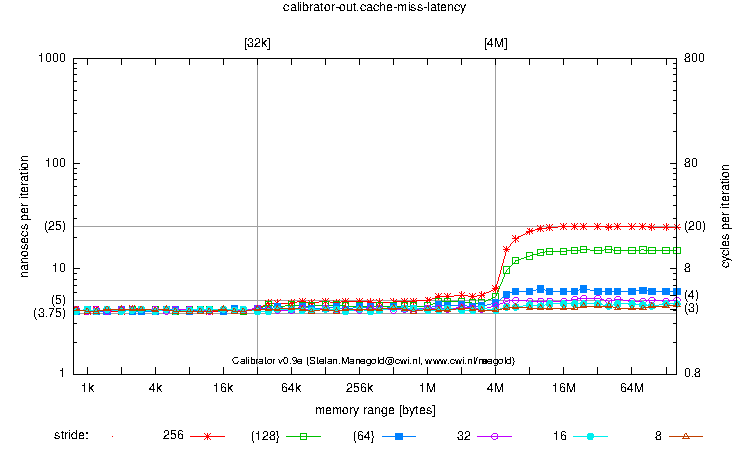
\includegraphics[type=pdf,ext=.pdf,read=.pdf,width=\columnwidth]{../system_info/calibrator-out.cache-miss-latency}
	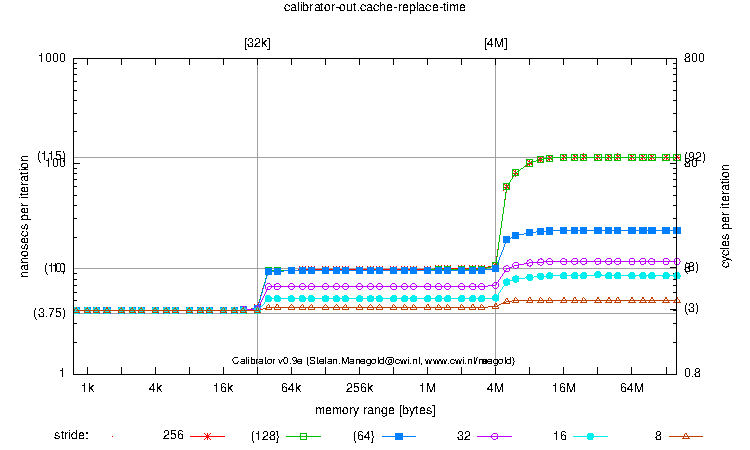
\includegraphics[type=pdf,ext=.pdf,read=.pdf,width=\columnwidth]{../system_info/calibrator-out.cache-replace-time}
  \caption{The Calibrator graphs indicating data cache sizes.}
  \label{fig:calibrator_cache}
\end{figure}

\begin{figure}[htbp]
  \centering
	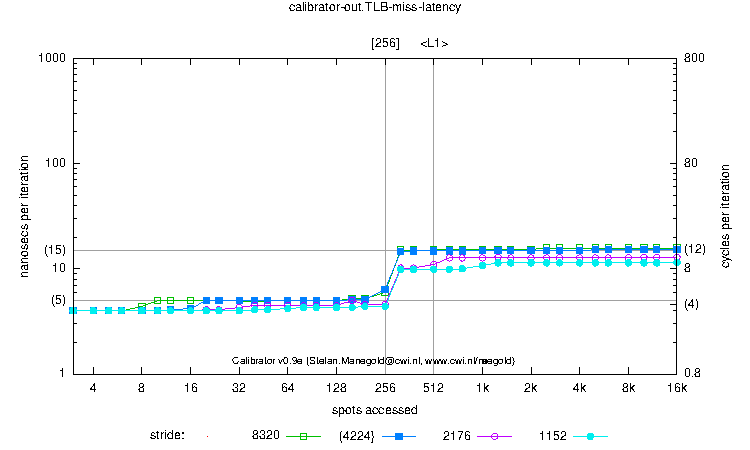
\includegraphics[type=pdf,ext=.pdf,read=.pdf,width=\columnwidth]{../system_info/calibrator-out.TLB-miss-latency}
  \caption{The Calibrator graph indicating TLB size.}
  \label{fig:calibrator_tlb}
\end{figure}

The Memory Organization Benchmark \cite{mob} was also run and further supported
the other tools. All of the system information gathered is in the
\texttt{system\_info} directory submitted with this report, notably in
\texttt{output.txt}.

\section{Summary of Experiments}

\subsection{Source Code}
The source code for each of the algorithms (with the exception of FFTW) can be
found in the included files.  The file {\tt four1.c} contains the iterative
implementation from \emph{Numerical Recipes in C}.  The file {\tt fft.c}
contains our implementations of both the na\"{i}ve and optimized versions of the
the radix-2 FFT algorithm.  Note that even though this source contains multiple
implementations of these algorithms, the functions named {\tt kd\_fftr2} and
{\tt kd\_fftr2\_opt} are the only ones we measured for comparisons.  The file
{\tt fft4.c} contains the FFT radix-4 code from ``How To Write Fast Numerical
Code: A Small Introduction''.

\subsection{Timing the Algorithms}

In order to measure the performance of each of the algorithms, we used the
Performance Application Programming Interface (PAPI) to record the following
metrics for each experiment:

\begin{itemize}
\item {\tt PAPI\_TOT\_CYC} - total cycles
\item {\tt PAPI\_TOT\_INS} - number of instructions completed
\item {\tt PAPI\_FP\_OPS}  - floating point operations
\item {\tt PAPI\_L1\_DCM}  - level 1 data cache misses
\end{itemize}

The file {\tt time\_fft.c} contains the main program which uses PAPI to compute
and report these statistics.  The included {\tt Makefile} should properly
compile all the source code and produce a program named {\tt time\_fft}.  This
program is used to generate the above statistics for the desired
implementation, input vector size, and number of times to repeatedly call the
indicated function.  The program also performs a simple test on the
implementation chosen to ensure that it has been implemented correctly.  The
output from the program is the average, minimum, and maximum values of each of
the above statistics.  For example, the following command generates these
statistics when the na\"{i}ve implementation of the FFT is called 10 times on a
vector of length $2^5$:
\begin{verbatim}
  time_fft 5 10 4 0
\end{verbatim}
The $4$ in the above command tells the program which of the functions to call
to perform the FFT.  To obtain a usage statement for the program which details
the allowable values for this argument, simply type {\tt time\_fft} at the
command line.  The $0$ in the above command indicates which test function to
run on the chosen function.  This will be explained momentarily.

The timings which we present in this report were computed by running the above
program on each of the implementations on input vectors of sizes $2^k$, where
$k$ ranged from $1$ to $24$ (with the exception of the radix 4 code whose input
sizes were of size $2^{2k}$, where $k$ ranged from $1$ to $12$).  Each function
was called 10 times on each input vector.  The included shell script {\tt
	time.sh} may be used to recreate the timing data, which is presented in its
raw format in the file timings.txt.

In addition to the raw data in timings.txt, we have also prepared performance
plots for all of the data collected to give a visual comparison of the
different algorithms.  Two such plots are presented below Figure
\ref{fig:ave_ops}, which compares the average number of floating point
operations performed by each of the algorithms on the smaller and larger input
sizes\footnote{Note that {\tt DFT\_rec} and {\tt DFT\_buf\_rec} refer to the
	radix-4 implementations of the FFT, without and with, respectively,
	buffering.}.

\begin{figure}[htbp]
  \centering
	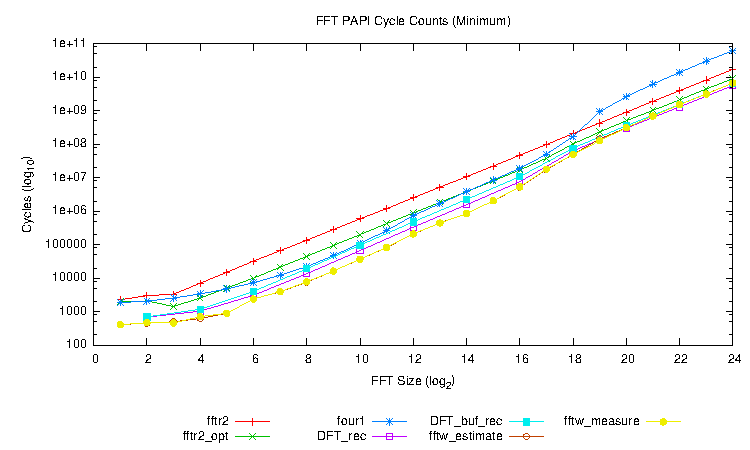
\includegraphics[width=\columnwidth]{../plots/tot_cyc_min}
	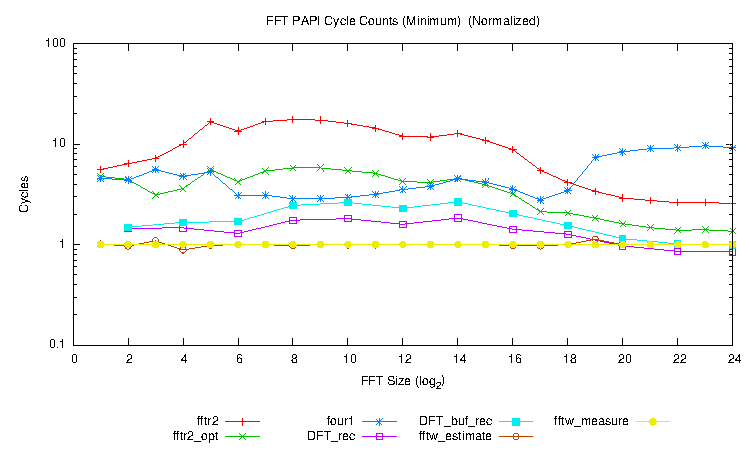
\includegraphics[width=\columnwidth]{../plots/tot_cyc_min_norm}
  \caption{}
  \label{fig:cyc_min}
\end{figure}

\begin{figure}[htbp]
  \centering
	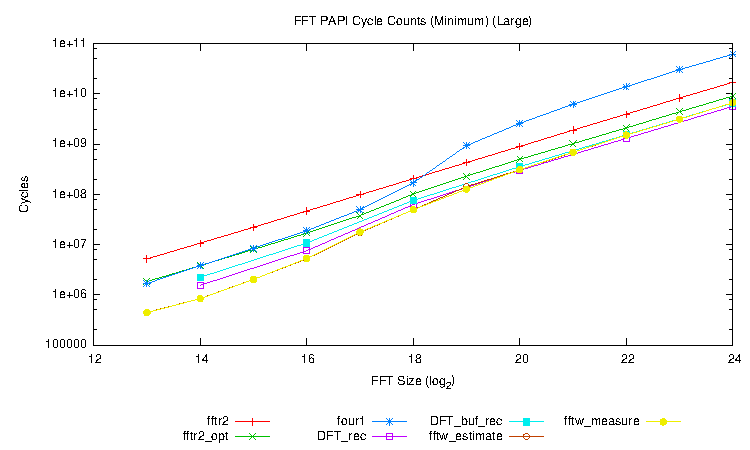
\includegraphics[width=\columnwidth]{../plots/tot_cyc_min_large}
	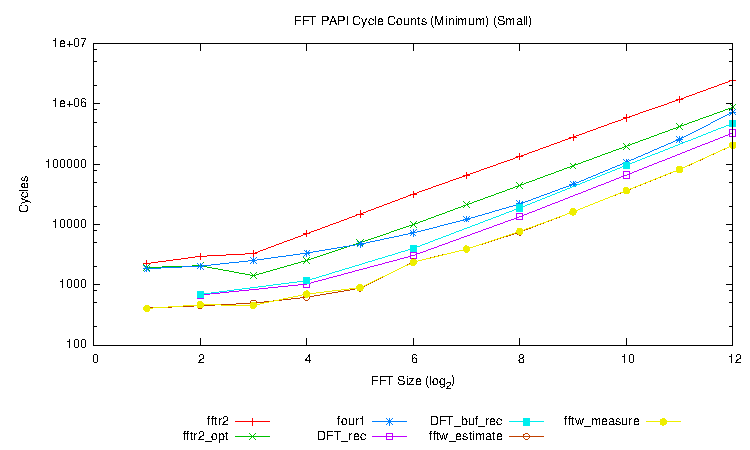
\includegraphics[width=\columnwidth]{../plots/tot_cyc_min_small}
  \caption{}
  \label{fig:cyc_min_size}
\end{figure}


\begin{figure}[htbp]
  \centering
	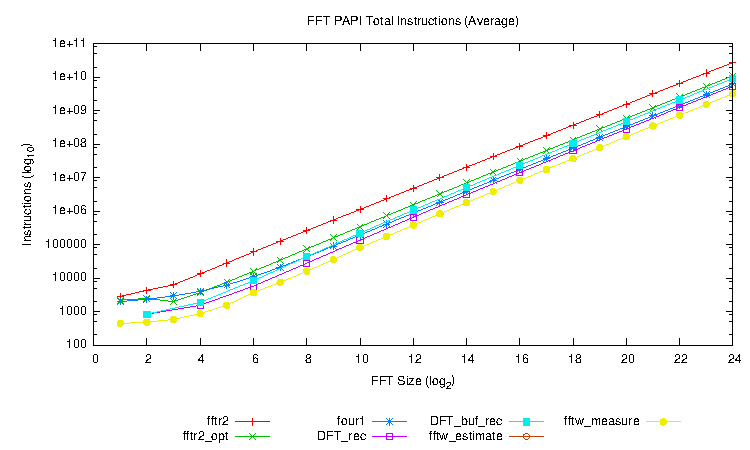
\includegraphics[width=\columnwidth]{../plots/tot_ins_ave}
	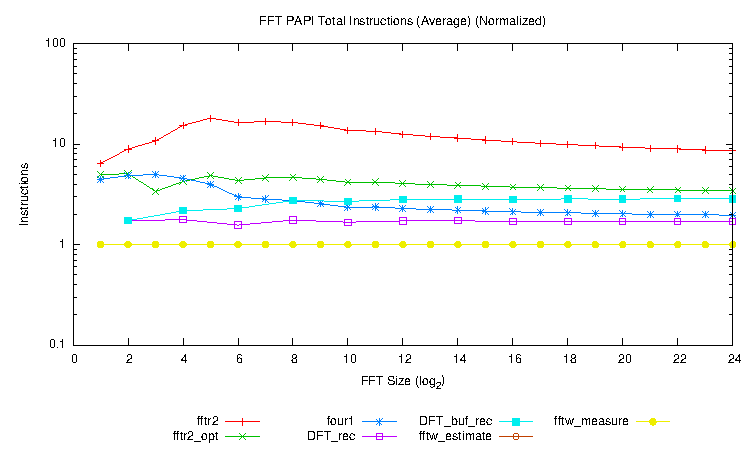
\includegraphics[width=\columnwidth]{../plots/tot_ins_ave_norm}
  \caption{}
  \label{fig:ins_ave}
\end{figure}


\begin{figure}[htbp]
  \centering
	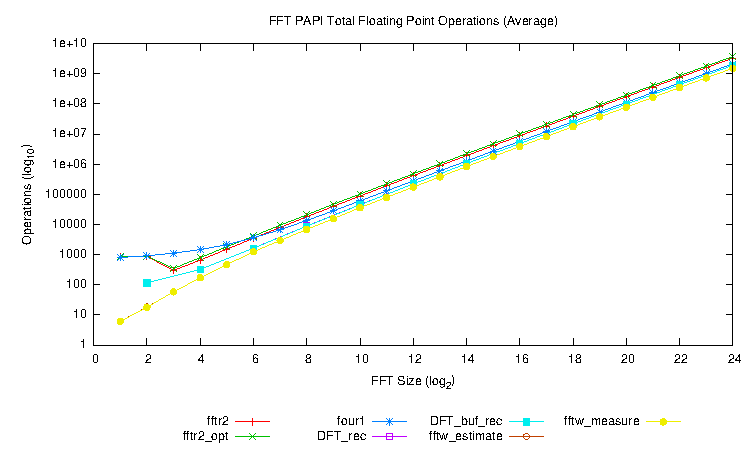
\includegraphics[width=\columnwidth]{../plots/fp_ops_ave}
	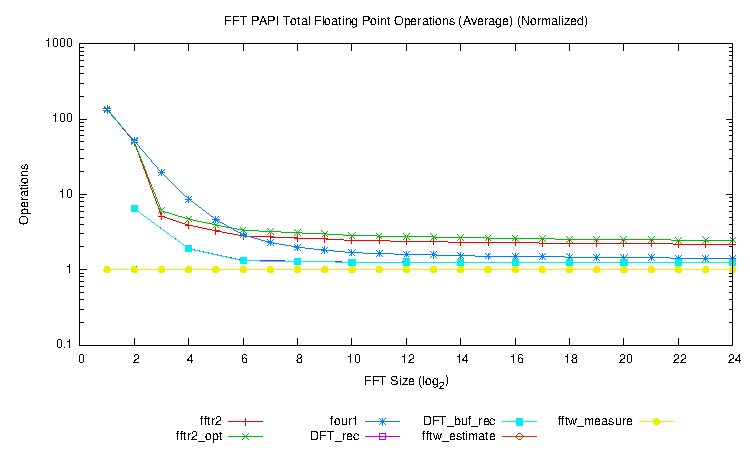
\includegraphics[width=\columnwidth]{../plots/fp_ops_ave_norm}
  \caption{Plot summary of the average number of floating point operations
		issued over 10 runs of each algorithm. The lower graph is normalized to the
		\texttt{fftw\_measure}. No major difference occurs when choosing the
		minimum instead of the average.}
  \label{fig:fp_ops}
\end{figure}

From Figure \ref{fig:fp_ops}, it seems quite clear that FFTW is by far the most
efficient implementation among those tested.  What is interesting here is how
little difference there appears to be between our na\"{i}ve implementation and
our optimized version.  Both of these implemenations appear to be relatively
inefficient.  However, some of the other plots (all of which are included in
the attached pdf files) do point out that the optimized version outperforms the
na\"{i}ve implementation in several areas.  For instance, Figure
\ref{fig:cache_misses_ave}) shows that not only does our optimized version produce
much fewer cache misses than our na\"{i}ve version, but out optimized version
actually outperforms all the other algorithms in this respect.

\begin{figure}[htbp]
  \centering
	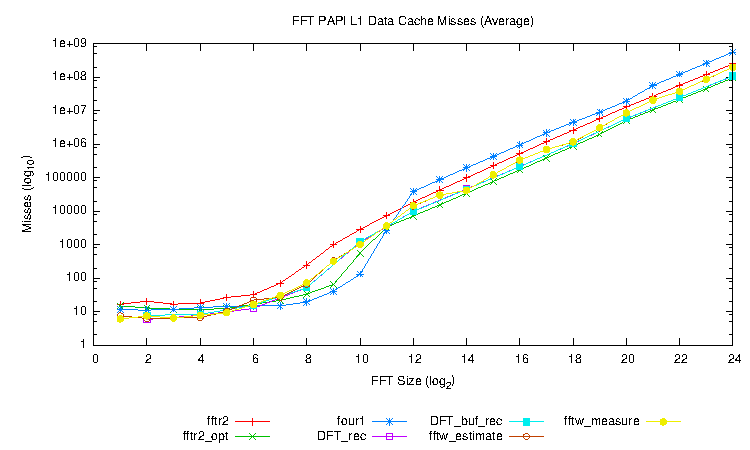
\includegraphics[width=\columnwidth]{../plots/l1dcm_ave}
	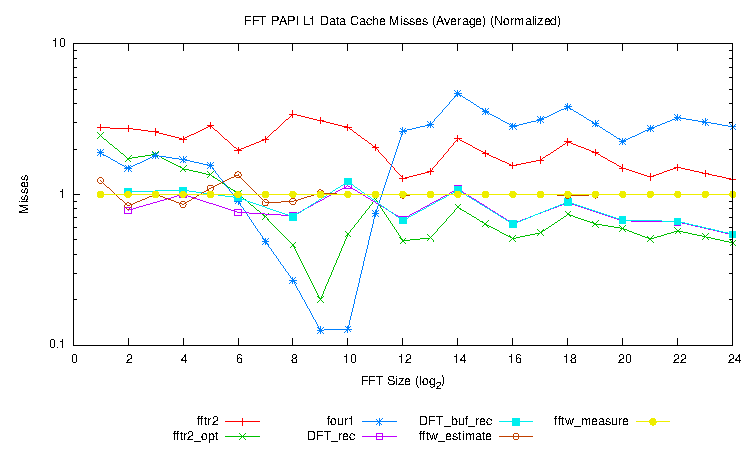
\includegraphics[width=\columnwidth]{../plots/l1dcm_ave_norm}
  \caption{Plot summary of the average number of cache misses encountered over
		10 runs of each algorithm on large input sizes.}
  \label{fig:cache_misses_ave}
\end{figure}

\begin{figure}[htbp]
  \centering
	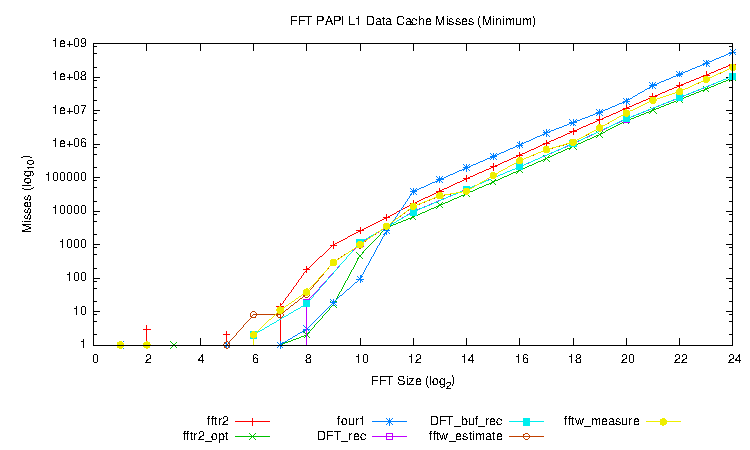
\includegraphics[width=\columnwidth]{../plots/l1dcm_min}
	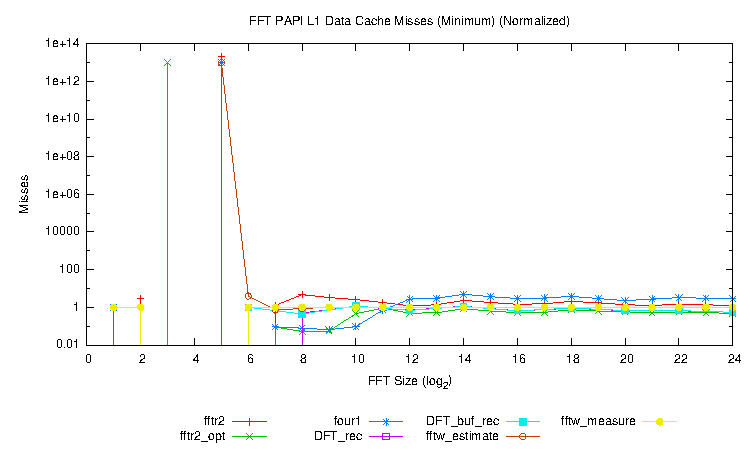
\includegraphics[width=\columnwidth]{../plots/l1dcm_min_norm}
  \caption{Plot summary of the minimum number of cache misses encountered over
		10 runs of each algorithm on large input sizes. The spikes in the
		normalized graph are due to the FFTW algorithm getting 0 cache misses
		during a run.}
  \label{fig:cache_misses_min}
\end{figure}

\subsection{Test Functions}
The file {\tt test.c} contains a suite of functions which can be used to ensure
that the various implementations of the FFT are working properly.  For each
test case, there are two functions, named {\tt test\emph{i}} and {\tt
	check\emph{i}}, for some integer $i$.  The {\tt test\emph{i}} function
creates an input vector of the desired size for which the output of the FFT is
known.  The {\tt check\emph{i}} function compares the output vector from that
FFT that it is given to the expected result.  The {\tt time\_fft} program can
be used to test the implementations by specifying an $i > 0$ as the final
command line argument.

\section{Conclusion}


\bibliographystyle{plain}
\bibliography{report}
\end{document}
